%!TEX root = ./book_omp.tex
% !TEX encoding = UTF-8 Unicode
%======================================================================================================================
% J.ROUSSEL
% 2019-09-11	 : création 
\setchapterstyle{kao}
\setchapterpreamble[u]{\margintoc}
\chapter{SÉRIE DE FOURIER}
\labch{serie-de-fourier}

En 1822, Joseph Fourier publie \emph{Théorie analytique de la chaleur}, ouvrage dans lequel il utilise une technique qui consiste à décomposer une fonction périodique par une somme infinie de sinus et de cosinus. Bien que suscitant quelques réserves de la part de nombreux mathématiciens de l'époque, l'analyse de Fourier est de nos jours solidement structurée et bien comprise. 

Ce chapitre explique cette décomposition spectrale et l'illustre dans le domaine de l'électronique et de la physique ondulatoire.

\begin{center}
\textbf{Version en ligne}

	\url{https://femto-physique.fr/omp/serie-de-fourier.php}
\end{center}


% =========================  partie I ===========================================================================

\section[Séries de Fourier]{Décomposition en séries de Fourier}%(fold)

\subsection{Signaux périodiques} % (fold)
De nombreux phénomènes se caractérisent par des signaux de différentes natures présentant une allure périodique. On peut penser au cycle des taches solaires, aux observables biologiques du corps humain (pression aortique, électrocardiogramme...), aux signaux électroniques, aux sons complexes produits par les instruments de musique, etc. Nous notons \(f(t)\) ce signal, et \(t\) une variable réelle. Pour fixer les idées, on peut imaginer que \(t\) soit la variable temporelle bien que ce ne soit pas nécessaire ; \(t\) peut aussi bien être une variable spatiale. Le signal admet \(T\) comme \textbf{période}\sidenote[][]{Notez que tout multiple de \(T\) est également une période ;  c'est pourquoi par convention la période est la plus petite valeur possible de \(T\) qui vérifie \eqref{serie-de-fourier-eq1}.}  lorsque l'on peut écrire 
\begin{equation}
f(t+T)=f(t)\quad\forall t \in \mathbb{R}
\quad\text{avec}\quad
T>0
\label{serie-de-fourier-eq1}
\end{equation}
\begin{marginfigure}[*0]
	\begin{tikzpicture}[scale=1]
		\begin{axis}[
			height=5cm,
			width=5cm,
			grid=major,
			axis lines=middle,% bottom,top
			inner axis line style={=>},
			xlabel style={anchor=west},
			ylabel style={anchor=east},
			xlabel={$t$},
			ylabel={$f(t)$},
			ymin=-.8,
			ymax=2,
			xmin=0,
			xmax=20,
			xtick=\empty,
			ytick={.5,.935},
			yticklabels={$f_\text{cc}$,$f_\text{rms}$},
			]
			\addplot+[mark=none,monBleu,domain=0:20,samples=250]{.5+sin(deg(x))+0.25*cos(3*deg(x))};
			\addplot+[mark=none,very thick,monBleu,domain=1.93:{2*pi+1.93},samples=50]{.5+sin(deg(x))+0.25*cos(3*deg(x))};
			\draw[|<->|](axis cs:1.93,1.8)--(axis cs:{2*pi+1.93},1.8)node[midway,fill=white]{$T$};
			\fill[lightgray,opacity=.5](axis cs:1.93,-2)rectangle(axis cs:{2*pi+1.93},2);
			\draw[gray,|<->|](axis cs:10,-.67)--(axis cs:10,1.66)node[pos=0.8,fill=white]{$f_\text{pp}$};
		\end{axis}
	\end{tikzpicture}
	\caption{Caractéristiques d'un signal périodique.}
	\labfig{SF1}
\end{marginfigure}
Toute l'information utile du signal se retrouve donc dans un motif de durée \(T\). Le nombre \(\nu\) de motifs que l'on trouve dans un intervalle d'une seconde s'appelle \textbf{la fréquence} et s'exprime en hertz (Hz). Vu que le motif s'étend sur une durée \(T\), on a
\begin{equation}
\fcolorbox{filet}{fond}{\hspace{0.5em}
\(\displaystyle
\nu=\frac{1}{T}
\)\hspace{0.5em}}
\hspace{0.5em}\heartsuit
\label{serie-de-fourier-eq2}
\end{equation}
Le motif présente des caractéristiques que l'on peut facilement mesurer dès lors que le signal est converti en un signal électrique :
\begin{itemize}
	\item La composante continue représente la valeur moyenne\sidenote[][*0]{La moyenne d'une fonction sur l'intervalle \([a,b]\) s'obtient par l'intégrale 
\[
	\overline{f}=\frac{1}{b-a}\int_{[a,b]}f(x)\, \mathrm{d}x
\]} du signal :
	\begin{equation}
		f_\text{cc}\stackrel{\text{def}}= \overline{f(t)}=\frac{1}{T}\int_{0}^{T}f(t)\,\mathrm{d}t
		\label{serie-de-fourier-eq3}
	\end{equation}

	\item La valeur crête-à-crête correspond à l'écart entre le maximum et le minimum de \(f\) :
	\begin{equation}
		f_\text{pp}\stackrel{\text{def}}=\max(f)-\min(f)
		\label{serie-de-fourier-eq4}
	\end{equation}
	\item Les signaux rencontrés en physique présentent une moyenne quadratique finie. En effet, la puissance d'un signal est proportionnelle à \(f^2(t)\) de sorte que sa moyenne doit être finie\sidenote[][]{On dit en mathématique que \(f\) est de carré sommable sur \([0,T]\).}. La valeur efficace\sidenote{en anglais \emph{rms-value} pour \emph{root mean square value}.} est liée à la moyenne quadratique \emph{via} la relation
	\begin{equation}
		f_\text{rms}\stackrel{\text{def}}= \sqrt{\overline{f^{2}}}= \sqrt{\frac{1}{T}\int_{0}^{T}f^2(t)\,\mathrm{d}t}
		\label{serie-de-fourier-eq5}
	\end{equation}
\end{itemize}
\begin{kaoexample}[frametitle=Exemple]
En électricité, la puissance électrique reçue par un conducteur ohmique de résistance \(R\) vaut \(\mathcal{P}(t)=Ri\,^2(t)\) de sorte que la puissance moyenne reçue vaut
\[
	\overline{\mathcal{P}}=R\, \overline{i^2}=R\, {i^2_\text{rms}}
\]
\end{kaoexample} 	
A priori, la fréquence et la valeur efficace d'un signal ne permettent pas de décrire complètement le signal périodique. En revanche, un sinus est complètement décrit par sa fréquence et sa valeur efficace ; il serait donc intéressant de pouvoir décomposer un signal périodique en sinus et cosinus.
% (end)
\subsection{Théorème de Fourier}% (fold)
\label{sec:theoreme_de_fourier}
\begin{marginfigure}[*1]
\includegraphics{./img/violon_Do3.png}
\caption{Note \(\mathsf{Do_3}\) jouée au violon.}
\labfig{note_do3_jouée_au_violon_}
\end{marginfigure}
Nous savons tous qu'une même note jouée sur un violon ou sur un piano sonne différemment bien que leurs fréquences sont identiques. En effet, l'oreille humaine, à l'instar d'un prisme avec la lumière, décompose les sons complexes en un spectre de sons purs que le cerveau est capable de comparer et d'interpréter. C'est l'idée de base de l'analyse de Fourier : décomposer un signal périodique de fréquence \(\nu\) en une somme de sinus de fréquences \textbf{multiples de \(\nu\)}. 
\begin{kaobox}[frametitle=Théorème de Fourier]
Sous certaines conditions mathématiques assez peu restrictives pour les grandeurs physiques, on montre qu'un signal périodique \(f(t)\) est développable en série de Fourier, comme suit :
\begin{equation}
f(t)=a_{0}+\sum_{n=1}^{\infty}a_{n}\cos(n\, 2\pi \nu\, t)+b_{n}\sin(n\, 2\pi \nu \, t)
\quad\text{avec}\quad
n\in \mathbb{N}
\label{serie-de-fourier-eq6}
\end{equation}
Le terme \(a_{n}\cos(n\, 2\pi \nu\, t)+b_{n}\sin(n\, 2\pi \nu \, t)\) représente l'\textbf{harmonique de rang} \(n\). L'harmonique de rang \(n=1\) est aussi appelée \textbf{le fondamental} de \(f\). 

\textbf{NB} : La série de Fourier converge point à point en \(f(t)\) si le signal est continu et d'énergie finie sur une période.
\end{kaobox}
L'ensemble des coefficients de Fourier \((a_n,b_n)\) détermine complètement la forme du motif périodique. C'est pourquoi, une autre façon de représenter un signal est de fournir l'histogramme des coefficients de Fourier : on obtient ce que l'on appelle la \textbf{représentation spectrale} ou le \textbf{spectre de Fourier} de \(f\). Par exemple, deux notes de même hauteur\sidenote{La hauteur est reliée à sa fréquence, par exemple un \(La_{440}\) correspond à un signal acoustique de fréquence 440~Hz} jouées par  deux instruments de musique différents présentent deux spectres constitués des mêmes harmoniques mais dont les poids relatifs diffèrent. Ces notes sont de hauteur identique mais de \textbf{timbre} distinct.

\begin{figure}
	\centering
	\begin{tikzpicture}[scale=1,font=\footnotesize]
		\begin{axis}[
		    title={Représentation temporelle},
			name=P1,
			width=6cm,
			xlabel={$t$},
			ylabel={$f(t)$},
			axis x line=middle,axis y line=middle,
			xlabel style={anchor=west},
			xmin=-1.2,xmax=1.2,ymin=-.75,ymax=3.25,
			ytick={1,3},
			yticklabels={1,3}
			]
			\addplot[domain=-1:1,color=monBleu,samples=200] {1+cos(360*\x)-.5*sin(360*2*\x)+.3*cos(360*4*\x)+.2*cos(360*6*\x) + .1*sin(360*9*\x) };
		\end{axis}
		\begin{axis}[
			name=P2,at={($(P1.east)+(20mm,0)$)},anchor=west,
			width=6cm,
		    title={Représentation spectrale},
			xlabel={\(n\)},xtick={1,2,3,4,5,6,7,8,9},xticklabels={1,2,3,4,5,6,7,8,9},
			ylabel={},
			axis x line=middle,axis y line=middle,
			grid=major,
			xmin=-.5,xmax=10,	ymin=-.6,ymax=1.2,
			]
			\addplot+[mark=*,mark options={draw=monBleu,fill=monBleu},monBleu,ycomb]  coordinates{(0,1) (1,1)  (4,.3) (6,.2) };
			\addlegendentry{\(a_n\)};
			\addplot+[monOrange,mark=*,mark options={draw=monOrange,fill=monOrange},ycomb]  coordinates{(2,-.5) (9,.1) };
			\addlegendentry{\(b_n\)};
		\end{axis}
	\end{tikzpicture}
	\caption{Passage de l'espace réel (temporel) à l'espace de Fourier (fréquentiel).}
	\labfig{SF2}
\end{figure}

\marginnote[*2]{On rappelle que les fonctions circulaires (sinus et cosinus) sont de moyenne nulle et de valeur efficace \(1/\sqrt{2}\). Plus généralement pour tout couple \((m,n)\) d'entiers non nuls, on a
\[
\overline{\sin(m\,x)\sin(n\, x)}=
\begin{cases}
\dfrac12&\text{si }m=n\\
0&\text{sinon}
\end{cases}
\]
et
\[
\overline{\sin(m\,x)\cos(n\, x)}=0
\]}

Si la fonction \(f(t)\) est connue, on peut déterminer les coefficients de Fourier par intégration. Par exemple, si l'on prend la moyenne de la série de Fourier on trouve \(a_0\). Le premier coefficient de Fourier représente donc la composante continue de \(f\) :
\begin{equation}
\fcolorbox{filet}{fond}{\hspace{0.5em}
\(\displaystyle
a_0=	f_\text{cc}=\frac{1}{T}\int_{0}^{T}f(t)\,\mathrm{d}t
\)\hspace{0.5em}}
\hspace{0.5em}\heartsuit
\label{serie-de-fourier-eq7}
\end{equation}

Quand on multiplie le développement de Fourier par \(\cos(n\, 2\pi \nu\, t)\) puis que l'on calcule la moyenne, tous les termes s'annulent sauf le terme \(a_n\overline{\cos^2(n\, 2\pi \nu\, t)}\) qui vaut \(a_n/2\). On en déduit\sidenote{Pour déterminer \(b_n\) il suffit de multiplier la série de Fourier par  \(\sin(n\, 2\pi \nu\, t)\) puis de prendre la moyenne temporelle.}
\begin{equation}
\fcolorbox{filet}{fond}{\hspace{0.5em}
\(\displaystyle
a_n=\frac{2}{T}\int_{0}^{T}f(t)\cos(n\, 2\pi \nu\, t)\,\mathrm{d}t
\quad\text{et}\quad
b_n=\frac{2}{T}\int_{0}^{T}f(t)\sin(n\, 2\pi \nu\, t)\,\mathrm{d}t
\)\hspace{0.5em}}
\hspace{0.5em}\heartsuit
\label{serie-de-fourier-eq8}
\end{equation}
	

%     * Idées de base [2][9][10]
%     * énoncé
%     * condition de convergence [2] [9]
%     * vocabulaire emprunté à la musique [9]p254
%     * spectre , les deux représentations : f(t) ->{an,bn}
%     * spectre de puissance
%     * exemple de spectre [8]

% (end)
\subsection{Illustration sur un exemple}\labsec{illustration_sur_un_exemple}%(fold)
Voyons par exemple comment un signal triangulaire se décompose en série de Fourier. Pour simplifier, prenons un signal triangulaire d'amplitude \(A\) et de période \(T=1\,\mathrm{s}\). Sa fréquence fondamentale est donc \(\nu=1\,\mathrm{Hz }\). En vertu du théorème de Fourier, le signal se développe comme suit :
\[
f(t)=a_0+\sum_{n=1}^\infty a_n\cos(2\pi n\, t)+b_n\sin(2\pi n\, t)
\]
\begin{marginfigure}[*-5]
\centering
\begin{tikzpicture}[scale=1]
	\begin{axis}[
		height=4cm,
		width=6cm,
		%grid=major,
		axis lines=middle,% bottom,top
		inner axis line style={=>},
		xlabel style={anchor=west},
		ylabel style={anchor=west},
		xlabel={$t$},ylabel={$f(t)$},
		ymin=-1.2,ymax=1.2,xmin=-1.2,xmax=1.2,
		xtick={-1,1},ytick={1,-1},yticklabels={\(A\),\(-A\)},
		]
		\draw[monBleu] (axis cs:-1.5,-1)--(axis cs:-1,1)--(axis cs:-.5,-1)--(axis cs:0,1)--(axis cs: .5,-1)--(axis cs:1,1)--(axis cs:1.5,-1);
	\end{axis}
\end{tikzpicture}
\caption{Signal triangulaire.}
\labfig{SF3}
\end{marginfigure}

Tout d'abord, le signal présente une composante continue nulle. Par conséquent \(a_0=0\). Ensuite, l'origine des temps est placé de telle sorte que la fonction est paire ; par conséquent le développement ne peut contenir que des harmoniques paires. C'est pourquoi les coefficients \(b_n\) sont tous nuls. Il ne nous reste plus qu'a déterminer les coefficients \(a_n\) donnés par
\marginnote[*3]{Rappelons que si \(f\) est paire, \[\int_{-a}^{a}f(x)\,\mathrm{d}x=2\int_{0}^{a}f(x)\, \mathrm{d}x\]}
\[
\begin{array}{rcl}
\dfrac{a_n}{2}	&=& \displaystyle{\int_{-1/2}^{1/2}}f(t)\cos(2\pi n\, t)\,\mathrm{d}t \\[4mm]
				&=& 2\displaystyle{\int_{0}^{1/2}}f(t)\cos(2\pi n\, t)\, \mathrm{d}t \\[4mm]
\dfrac{a_n}{2}	&=& 2\displaystyle{\int_{0}^{1/2}}(A-4At)\cos(2\pi n\, t)\, \mathrm{d}t
\end{array}
\]
où \(f(t)\) a été remplacée par la portion de droite d'équation \(A-4At\) entre \(t=0\) et \(t=\frac12\). On poursuit le calcul en intégrant par partie :
\[
\begin{array}{rcccl}
\dfrac{a_n}{2}	&=&2\left[(A-4At)\dfrac{\sin(2\pi n \,t)}{2\pi n}\right]_0^{1/2}&+&2\displaystyle{\int_{0}^{1/2}}\dfrac{4A\sin(2\pi n \,t)}{2\pi n}\, \mathrm{d}t \\[4mm]
			&=&0&+&	2\left[-\dfrac{4A\cos(2\pi n \,t)}{(2\pi n)^2}\right]_0^{1/2}\\[4mm]
\dfrac{a_n}{2}	&=&\dfrac{2A}{\pi^2n^2}\left(1-\cos(\pi n)\right)&&\\
\end{array}
\]
Sachant que \(\cos(\pi n)=(-1)^n\), on trouve finalement
\begin{equation}
	a_n=
	\begin{cases}
	0					& \text{si } n \text{ est pair} \\[3mm]
	\dfrac{8A}{\pi^2} \dfrac{1}{n^2},	& \text{si } n \text{ est impair.}
	\end{cases}
	\quad\text{et}\quad
	b_n=0
	\label{coef_fourier_triangle}
\end{equation}
Autrement dit, le signal triangulaire est exclusivement constitué d'harmoniques de fréquences multiples impaires de la fréquence fondamentale et dont les amplitudes décroissent assez rapidement. La huitième composante par exemple correspond à \(n=15\) et présente une amplitude 225 fois plus faible que celle du fondamental.
\begin{marginfigure}[*-10]
\centering
\begin{tikzpicture}
	\begin{axis}[
		width=5cm,
		height=5cm,
		xlabel={\(n\)},xtick={0,1,2,3,4,5,6,7,8,9},
		ylabel={\(a_n\)},
		ytick={0,1},
		yticklabels={0,\(\frac{8A}{\pi^2}\)},
		axis x line=middle,axis y line=middle,
		xlabel style={anchor=west},
		ylabel style={anchor=south},
		% grid=major,
		xmin=0,xmax=10,	ymin=0,ymax=1.1,
		font=\footnotesize
		]
		\addplot+[monBleu,mark options={draw=monBleu,fill=monBleu},ycomb]  coordinates{(0,0) (1,1) (3,{1/9}) (5,{1/25}) (7,{1/49}) (9,{1/81})};
	\end{axis}
\end{tikzpicture}
\caption{Spectre du signal triangulaire}
\labfig{SF4}
\end{marginfigure}
On comprend dès lors que la convergence de la série de Fourier est ici assez rapide comme le montre la figure ci-dessus.
\begin{figure*}[h!btp]
\centering
\begin{tikzpicture}[scale=1]
	\begin{axis}[name=P1,height=5cm,width=5cm,title={1 harmonique},xlabel={$t$},ylabel={$f(t)$},grid=major,axis x line=middle,axis y line=middle,xmin=-1.2,xmax=1.2,ymin=-1.4,ymax=1.4,xtick={-.5,.5},xticklabels={$-1$,$1$},ytick={-1,1},yticklabels={$-A$,$A$},,font=\footnotesize]
	%\draw[monBleu,dashed] (axis cs:-1,1)--(axis cs:-.5,-1)--(axis cs:0,1)--(axis cs: .5,-1)--(axis cs:1,1);
	\addplot[domain=-1:1,color=monBleu,samples=400] {.811*(cos(360*\x))};
	\end{axis}
	\begin{axis}[name=P2,at={($(P1.east)+(5mm,0)$)},anchor=west,height=5cm,width=5cm,title={2 harmoniques},xlabel={$t$},ylabel={$f(t)$},grid=major,axis x line=middle,axis y line=middle,xmin=-1.2,xmax=1.2,ymin=-1.4,ymax=1.4,xtick={-.5,.5},xticklabels={$-1$,$1$},ytick={-1,1},yticklabels={$-A$,$A$},,font=\footnotesize]
	%\draw[monBleu,dashed] (axis cs:-1,1)--(axis cs:-.5,-1)--(axis cs:0,1)--(axis cs: .5,-1)--(axis cs:1,1);
	\addplot[domain=-1:1,color=monBleu,samples=400] {.811*(cos(360*\x)+(1/9)*cos(360*3*\x))};
	\end{axis}
	\begin{axis}[name=P3,at={($(P2.east)+(5mm,0)$)},anchor=west,height=5cm,width=5cm,title={4 harmoniques},xlabel={$t$},ylabel={$f(t)$},grid=major,axis x line=middle,axis y line=middle,xmin=-1.2,xmax=1.2,ymin=-1.4,ymax=1.4,xtick={-.5,.5},xticklabels={$-1$,$1$},ytick={-1,1},yticklabels={$-A$,$A$},,font=\footnotesize]
	%\draw[monBleu,dashed] (axis cs:-1,1)--(axis cs:-.5,-1)--(axis cs:0,1)--(axis cs: .5,-1)--(axis cs:1,1);
	\addplot[domain=-1:1,color=monBleu,samples=400] {.811*(cos(360*\x)+(1/9)*cos(360*3*\x)+(1/25)*cos(360*5*\x)+(1/49)*cos(360*7*\x))};
	\end{axis}
	\begin{axis}[name=P4,at={($(P3.east)+(5mm,0)$)},anchor=west,height=5cm,width=5cm,title={8 harmoniques},xlabel={$t$},ylabel={$f(t)$},grid=major,axis x line=middle,axis y line=middle,xmin=-1.2,xmax=1.2,ymin=-1.4,ymax=1.4,xtick={-.5,.5},xticklabels={$-1$,$1$},ytick={-1,1},yticklabels={$-A$,$A$},,font=\footnotesize]
	%\draw[monBleu,dashed] (axis cs:-1,1)--(axis cs:-.5,-1)--(axis cs:0,1)--(axis cs: .5,-1)--(axis cs:1,1);
	\addplot[domain=-1:1,color=monBleu,samples=400] {.811*(cos(360*\x)+(1/9)*cos(360*3*\x)+(1/25)*cos(360*5*\x)+(1/49)*cos(360*7*\x) + (1/81)*cos(360*9*\x) + (1/121)*cos(360*11*\x) + (1/169)*cos(360*13*\x) + (1/225)*cos(360*15*\x))};
	\end{axis}
\end{tikzpicture}
\caption[Approximation du signal triangulaire]{Approximation du signal triangulaire en tronquant la série de Fourier à \(n=1,3,7\) et 15.}
\labfig{serie-de-fourier-fig4}
\end{figure*}

%     * calcul des an, bn, An, sur un signal triangulaire [2]
%     * simu (on montre la convergence)
%(end)
\subsection{Notation complexe}%(fold)
On peut reformuler le développement de Fourier en notation complexe. À partir de \eqref{serie-de-fourier-eq6} et des relations d'Euler, on a 
\[
\begin{array}{ccl}
f(t)	&=&	a_0+\displaystyle{\sum_{n=1}^\infty a_n\frac{\mathrm{e}^{i n\,2\pi\nu\, t}+\mathrm{e}^{-i n\,2\pi\nu\, t}}{2}+b_n\frac{\mathrm{e}^{i n\,2\pi\nu\, t}-\mathrm{e}^{-i n\,2\pi\nu\, t}}{2i}}\\[3mm]
	&=&a_0+\displaystyle{\sum_{n=1}^\infty \frac{a_n-ib_n}{2}\,\mathrm{e}^{i n\,2\pi\nu\, t}+ \frac{a_n+ib_n}{2}\,\mathrm{e}^{-i n\,2\pi\nu\, t}}\\[3mm]
f(t)	&=& 	\displaystyle{\sum_{n=-\infty}^\infty \underline{c_n}\,\mathrm{e}^{i n\,2\pi\nu\, t}}
\end{array}
\]
\marginnote[*-2]{\textbf{Attention}, la somme s'étend sur \(\mathbb{Z}\)!}
où \(\underline{c_n}\) est le \textbf{coefficient de Fourier complexe} donné par
\[
\underline{c_n} \stackrel{\text{def}}= 
\begin{cases}
\dfrac{a_n-ib_n}{2} & \text{si } n>0 \\
\underline{c_{-n}}^\star & \text{si } n<0
\end{cases}
\qquad\text{et}\qquad
c_0 \stackrel{\text{def}}= a_0
\] 
Si l'on reprend les relations \eqref{serie-de-fourier-eq8}, on s'aperçoit que le coefficient de Fourier complexe se calcule via la formule 
\begin{equation}
\fcolorbox{filet}{fond}{\hspace{0.5em}
\(\displaystyle 
\underline{c_n}=\frac{1}{T}\int_{0}^{T}f(t) \, \mathrm{e}^{-i n\,2\pi\nu\, t}\,\mathrm{d}t
\quad\text{avec}\quad n\in \mathbb{Z}
\)\hspace{0.5em}}
\hspace{0.5em}\heartsuit
\label{serie-de-fourier-eq9}
\end{equation}
L'ensemble  des modules des \(\underline{c_n}\) constitue le spectre de \(f\) en \emph{amplitude}, alors que l'ensemble des arguments des \(\underline{c_n}\) donne le spectre en phase. Pour un signal réel on a \(\underline{c_{-n}}=\underline{c_n}^\star\), soit \(|\underline{c_{-n}}|=|\underline{c_n}|\) et \(\arg(\underline{c_{-n}})=-\arg(\underline{c_n})\). Autrement dit, le spectre en amplitude est symétrique par rapport à l'axe \(n=0\), le spectre en phase anti-symétrique. Pour ces raisons, on se contente souvent de représenter les spectres pour les valeurs positives de \(n\).


%     * formulation complexe du Théorème de fourier [3]
%     * expression de cn [3]1
%     * Propriété de cn pour un signal réel
%     * spectre d’amplitude : on ne représente que la moitié car |cn| est pair
%(end)
\subsection{Relation de Parseval}%(fold)
La puissance moyenne du signal \(f(t)\) est proportionnelle au carré de sa valeur efficace. Or, chaque harmonique transporte également une puissance proportionnelle à sa valeur efficace. La relation de Parseval exprime simplement le fait que la puissance du signal est égale à la somme des puissances transportées par les différentes harmoniques, ce qui en terme de valeurs efficace se traduit\sidenote[][*0]{On rappelle qu'un signal sinusoïdal d'amplitude \(a\) présente une valeur efficace égale à \(a/\sqrt{2}\). Quant au signal constant d'amplitude \(a\) sa valeur efficace vaut également \(a\).} par la relation
\begin{equation}
\fcolorbox{filet}{fond}{\hspace{0.5em}
\(\displaystyle 
\overline{f^2}\stackrel{\text{def}}= f^2_\text{rms}=a_0^2+\sum_{n=1}^\infty \frac{a_n^2+b_n^2}{2}
\)\hspace{0.5em}}
\hspace{0.5em}\heartsuit
\label{serie-de-fourier-eq10}
\end{equation}
La relation \eqref{serie-de-fourier-eq10} prend une forme particulièrement simple lorsque l'on fait intervenir les coefficients de Fourier complexes. En effet, sachant que \(c_{n>0}=\frac12 (a_n-ib_n)=c^\star_{n<0}\) et \(c_0=a_0\), on obtient
\begin{equation}
\fcolorbox{filet}{fond}{\hspace{0.5em}
\(\displaystyle 
\overline{f^2}=\sum_{n=-\infty}^\infty |c_n|^2
\)\hspace{0.5em}}
\hspace{0.5em}\heartsuit
\label{serie-de-fourier-eq11}
\end{equation}
\begin{kaoexample}[frametitle=Démonstration du théorème de Parseval]
Le développement de Fourier \eqref{serie-de-fourier-eq6} peut aussi s'écrire  : 
\[
f(t)=a_{0}+\sum_{n=1}^{\infty}A_{n}\cos(n\, 2\pi \nu\, t+\varphi_n)
\quad\text{avec}\quad
A_n^2=a_n^2+b_n^2
\quad\text{et}\quad
n\in \mathbb{N}
\]
où \(A_n\) représente l'amplitude de l'harmonique de rang \(n\). Élevons au carré le signal :
\[
	\begin{array}{ccccc}
		f^2(t)	&=&a_0^2&+&2a_0\sum_{n=1}^{\infty}A_{n}\cos(n\, 2\pi \nu\, t+\varphi_n)\\[1mm]
				&&&+&\sum_{n,m}A_nA_{m}\cos(n\, 2\pi \nu\, t+\varphi_n)\cos(m\, 2\pi \nu\, t+\varphi_m)
	\end{array}
\]
Calculons maintenant la moyenne de \(f^2(t)\) sur une période. Compte tenu des propriétés des fonctions trigonométriques, on obtient 
\[
\overline{f^2}=a_0^2+\sum_{n=1}^\infty \frac{A_n^2}{2}=a_0^2+\sum_{n=1}^\infty \frac{a_n^2+b_n^2}{2}
\]
\end{kaoexample} 
\begin{marginfigure}
\centering
\begin{tikzpicture}
	\begin{axis}[
		width=6cm,
		xlabel={\(n\)},
		ylabel={\(|c_n|\)},
		axis x line=middle,axis y line=middle,xlabel style={anchor=west},
		minor tick num=4,
		grid=both,
		xmin=-8,xmax=8,	ymin=0,ymax=1.2,
		font=\footnotesize
		]
		\addplot+[monBleu,mark options={draw=monBleu,fill=monBleu},ycomb]  coordinates{(-1,.6)  (-2,.25) (-4,.2) (-6,.1) (-7,.1) (0,1) (1,.6)  (2,.25) (4,.2) (6,.1) (7,.1) };
	\end{axis}
\end{tikzpicture}
\caption{Spectre de \(u(t)\)}
\labfig{spectre_d_amplitude_du_signal}
\end{marginfigure}

\exercice{On enregistre à l'oscilloscope une tension électrique \(u(t)\) dont on donne le spectre en amplitude. On envoie cette tension aux bornes d'un voltmètre en mode AC. Quelle valeur affiche-t-il sachant que sa résolution est de 10~mV ?\\
\emph{Rép.}~~Le voltmètre affiche 0{,}98~V.}
%(end)

% (end)

% =====================  partie II =============================================================

\section{Applications}%(fold)

\subsection{Filtrage analogique} % (fold)
\labsec{filtrage_analogique}
Considérons un système qui transforme un signal d'entrée \(e(t)\) en un signal de sortie \(s(t)\). On appelle \textbf{filtre} un tel système si :
\begin{marginfigure}[*-1]
\centering
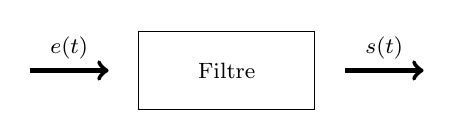
\begin{tikzpicture}[scale=1,font=\footnotesize]
	\draw[->,ultra thick,shift={(-2,0)}](-.5,0)--(.5,0)node[midway,above]{\(e(t)\)};
	\draw[->,ultra thick,shift={(2,0)}](-.5,0)--(.5,0)node[midway,above]{\(s(t)\)};
	\node[rectangle, minimum height=1cm, draw=black,text centered, text width=2cm, text centered] {Filtre};
\end{tikzpicture}
\caption{Filtre}
\labfig{filtre}
\end{marginfigure}
\begin{itemize}
	\item ses caractéristiques sont invariantes dans le temps;
	\item son comportement respecte le principe de superposition.
\end{itemize}
\marginnote[*1]{On adopte la notation complexe : \(\underline{e}(t)=\underline{E}\,\mathrm{e}^{i\, 2\pi\nu t}\)  et \(\underline{s}(t)=\underline{S}\,\mathrm{e}^{i\, 2\pi\nu t}\).}Un filtre est caractérisé par sa \textbf{fonction de transfert} 
\[
\underline{H}\stackrel{\text{def}}= \frac{\underline{s}(t)}{\underline{e}(t)}
\]
qui donne la réponse en régime sinusoïdal.

\begin{marginfigure}
\centering
\begin{tikzpicture}[scale=0.8,decoration={markings,mark=at position 5mm with {\arrowreversed{stealth};}},font=\footnotesize]
	\def \la {2};%largeur de l'AO
	\def \lo {2.25};%longueur de l'AO
	\coordinate (O) at (0,0);
	\coordinate (A) at ({-0.5*\lo},{-0.5*\la});
	\coordinate (B) at ({-0.5*\lo},{0.5*\la});
	\coordinate (C) at ({0.5*\lo},{0.5*\la});
	\coordinate (D) at ({0.5*\lo},{-0.5*\la});
	\coordinate (P) at ({-0.5*\lo},{-0.25*\la});%entrée1
	\coordinate (M) at ({-0.5*\lo},{0.25*\la});%entrée2
	\coordinate (S1) at ({0.5*\lo},{-0.25*\la});%sortie1
	\coordinate (S2) at ({0.5*\lo},{0.25*\la});%sortie2
	\draw[thick,rounded corners] (A)--(B)--(C)--(D)--cycle;
	\draw (O) node{Quadripôle};
	\draw (B)node[above left]{Entrée};
	\draw (C)node[above right]{Sortie};
	\draw[thin,postaction={decorate}] (M)--++(-1,0)node[midway,above]{$i_\text{e}$};
	\draw[thin] (P)--++(-1,0);
	\draw[thin,postaction={decorate}] (S2)++(1,0)--(S2) node[midway,above]{$i_\text{s}$};
	\draw[thin] (S1)++(1,0)--(S1);
	\draw[->] ({-\lo-0.1},{-0.25*\la})--++(0,{0.5*\la})node[midway, left]{$u_\text{e}$};
	\draw[->] ({\lo+0.1},{-0.25*\la})--++(0,{0.5*\la})node[midway, right]{$u_\text{s}$};
\end{tikzpicture}
\caption{Quadripôle électronique}
\labfig{Quadripole-electronique}
\end{marginfigure}
En électronique, dans une chaîne d'analyse et de traitement du signal électrique, on rencontre couramment des filtres sous la forme de quadripôles, c'est-à-dire d'éléments possédant deux bornes d'entrée et deux bornes de sortie. Les grandeurs d'entrée et de sortie sont les tensions ou les courants. La fonction de transfert correspond en général à la \emph{réponse en tension en boucle ouverte}\sidenote{C'est-à-dire lorsque la sortie ne débite aucun courant, comme c'est le cas lorsqu'on y branche un voltmètre ou un oscilloscope dont les impédances d'entrée sont suffisamment grandes pour être considérées infinies.} :
\begin{equation}
	\underline{H}(\nu)\stackrel{\text{def}}= \left.\frac{\underline{u_s}(t)}{\underline{u_e}(t)}\right|_{\underline{i_s}=0}
\end{equation}
\(\underline{H}\) est une grandeur complexe qui varie avec la fréquence, ou la \textbf{pulsation}\sidenote{La pulsation s'exprime en rad/s.} \(\omega=2\pi \nu\) selon les préférences.
Le module de la fonction de transfert renseigne sur le gain en amplitude \(G\) alors que l'argument donne le déphasage sortie/entrée \(\phi\): 
\begin{equation}
G\stackrel{\text{def}}= |\underline{H}|=\frac{S_\text{rms}}{E_\text{rms}}
\quad\text{et}\quad
\phi=\arg{\underline{H}}
\end{equation} 
\begin{marginfigure}[*3]
	\centering
	\begin{tikzpicture}[font=\footnotesize]
		\draw[dashed] (-1.25,-1)rectangle (1.25,1.5);
		\draw[thick] (-1.5,-.75)--(1.5,-.75);
		\draw[thick] (-1.5,.75)--(1.5,.75)(.75,.75)--++(0,-2.25)++(10pt,0)--++(-20pt,0);
		\fill[pattern=north east lines,opacity=0.6](.75cm-10pt,-1.5) rectangle (.75cm+10pt,-1.5cm-5pt);
		\resistanceV{shift={(.75,0)}}{$R$};
		\condoH{shift={(-1,.75)}}{$C$}{};
		\bobineH{shift={(0,.75)}}{$L$}{};
		\draw[shift={(2,-0.7)},->] (0,0)--++(0,1.4) node[midway,right]{$s(t)$};
		\draw[shift={(-2,-0.7)},->] (0,0)--++(0,1.4) node[midway,left]{$e(t)$};
	\end{tikzpicture}
\caption{Filtre RLC}
\labfig{filtre_rc}
\end{marginfigure}
\begin{kaoexample}[frametitle=Exemple : filtre RLC]
Étudions le filtre formé par la mise en série d'un conducteur ohmique de résistance \(R\), d'un condensateur de capacité \(C\) et d'une bobine de self-inductance \(L\). Le signal d'entrée sera la tension aux bornes de l'ensemble et le signal de sortie la tension aux bornes du conducteur ohmique. Nous reconnaissons un diviseur de tension, de sorte qu'en régime sinusoïdal on peut écrire\footnote{Rappelons qu'en électricité on convient de remplacer le nombre complexe \(i\) par \(j\) pour éviter les confusions avec l'intensité électrique.}
\[
\underline{s}(t)=\frac{\underline{Z}_R}{\underline{Z}_R+\underline{Z}_C+\underline{Z}_L}\underline{e}(t)
\quad\text{avec}\quad
\underline{Z}_R=R
\quad
\underline{Z}_L=jL\omega
\quad\text{et}\quad
\underline{Z}_C=\frac{1}{jC\omega}
\]
On en déduit le la fonction de transfert de ce filtre
\[
\underline{H}=\frac{\underline{s}(t)}{\underline{e}(t)}=\frac{1}{1+j\left(\frac{L\omega}{R}-\frac{1}{RC\omega}\right)}
\quad\text{avec}\quad
\omega=2\pi \nu
\]
\end{kaoexample} 
Souvent, le filtre présente un gain significatif pour un certain intervalle de fréquences alors qu'il est quasiment nul pour les autres fréquences. Le filtre élimine alors certaines harmoniques du signal. Suivant l'allure du gain avec la fréquence on distingue différents types de filtre :
\begin{itemize}
\item Le \textbf{filtre passe-bas} laisse passer les basses fréquences et coupe les hautes fréquences ;
\item Le \textbf{filtre passe-haut} laisse passer les hautes fréquences et coupe les basses fréquences ;
\item Le \textbf{filtre passe-bande} laisse passer les harmoniques situées dans une certaine bande de fréquences ;
\item Le \textbf{filtre réjecteur de bande} coupe les harmoniques dans une certaine bande de fréquences.
\end{itemize}
\begin{figure*}[htbp]
\centering
\begin{tikzpicture} [font=\footnotesize]
	\def \facteurQ {8}
	\begin{axis}[
		name=plot0,
		height=3cm,
		width=3cm,
		grid=major,
		axis lines=middle,% bottom,top
		inner axis line style={=>},
		xlabel={$\nu$},
		ylabel={Gain $G$},
		xtick=\empty,
	 	ytick=\empty,
		ymin=0,
		ymax=1,
		xmin=0,
		xmax=1,]
	\end{axis}
	\begin{axis}[
		name=plot1,
		at={($(plot0.east)+(1cm,0)$)},anchor=west,
		height=3cm,
		width=3cm,
	  title= Passe-Bas,
		xtick=\empty,
	 	ytick=\empty,
		ymin=0,
		ymax=1.5,
		xmin=0,
		xmax=3,]
		\addplot+[monBleu,mark=none,domain=0:5,samples=100]{1/(1+(\x*\x*\x))};
	\end{axis}
	\begin{axis}[
		name=plot2,
		at={($(plot1.east)+(1cm,0)$)},anchor=west,
		height=3cm,
		width=3cm,
	  title= Passe-Haut,
		xtick=\empty,
	 	ytick=\empty,
		ymin=0,
		ymax=1.5,
		xmin=0,
		xmax=3,]
		\addplot+[monBleu,mark=none,domain=0:5,samples=100]{\x/sqrt(1+(\x*\x))};
	\end{axis}
	\begin{axis}[
		name=plot3,
		at={($(plot2.east)+(1cm,0)$)},anchor=west,
		height=3cm,
		width=3cm,
	  title= Passe-Bande,
	 	xtick=\empty,
	 	ytick=\empty,
		ymin=0,
		ymax=9,
		xmin=0,
		xmax=3,]
		\addplot+[monBleu,mark=none,domain=0:3,samples=100]{1/sqrt((1-\x*\x)*(1-\x*\x)+(\x/\facteurQ)*(\x/\facteurQ))};
	\end{axis}
	\begin{axis}[
		name=plot4,
		at={($(plot3.east)+(1cm,0)$)},anchor=west,
		height=3cm,
		width=3cm,
	  title= Coupe-Bande,
	 	xtick=\empty,
	 	ytick=\empty,
		ymin=0,
		ymax=1.5,
		xmin=0,
		xmax=3,]
		\addplot+[monBleu,mark=none,domain=0:3,samples=100]{abs(1-\x*\x)/sqrt((1-\x*\x)*(1-\x*\x)+0.1*\x*\x)};
	\end{axis}
\end{tikzpicture}
\caption{Types de filtre souvent rencontrés.}
\labfig{types_de_filtres}
\end{figure*}
Lorsque l'on injecte en entrée d'un filtre un signal périodique, chaque harmonique de rang \(n\)  est atténuée d'une quantité \(G_n=G(n\nu)\) et déphasée de \(\phi_n=\phi(n\nu)\). En vertu du principe de superposition, on reconstitue le signal de sortie en sommant chaque harmonique une fois transformée par le filtre. Formellement, si \(a_n\) et \(b_n\) sont les coefficients de Fourier du signal d'entrée, alors le signal de sortie s'écrit
\[
s(t)=G_0a_0+\sum_{n=1}^\infty G_n\,a_n\cos\left[n\,2\pi\nu\, t+\phi_n\right]+
\sum_{n=1}^\infty G_n\,b_n\sin\left[n\,2\pi\nu\, t+\phi_n\right]
\]
\begin{marginfigure}
	\centering
	\begin{tikzpicture}
		\begin{axis}[
		width=6cm,
		title={$G=f(\nu)$},
		grid=major,
		xtick={1},
		xticklabels={\(\nu_0\)},
		ytick={1,.707},
		yticklabels={\(G_\text{max}\),\(\frac{G_\text{max}}{\sqrt{2}}\)},
		xmin=0,xmax=3,
		ymin=0,ymax=1.2,
		font=\footnotesize,
		clip=false,
		]
		\addplot[monBleu,domain=0:3,samples=200,]  {1/sqrt(1+25*(x-1/x)^2)};
		\addplot[thick,monBleu,fill=monBleu,opacity=0.2,domain=.9:1.1,samples=200]  {1/sqrt(1+25*(x-1/x)^2)}\closedcycle;
		\draw[->|] (axis cs:.7,.707)--(axis cs:.9,.707);
		\draw[|<-] (axis cs:1.1,.707)--(axis cs:1.3,.707)node[right,fill=white]{bande-passante \(\Delta\nu\)};
	\end{axis}
	\end{tikzpicture}
	\caption{Courbe de réponse du circuit RLC.}
	\labfig{courbe_de_reponse_d_un_circuit_rlc}
\end{marginfigure}
Pour illustrer notre propos considérons le filtre RLC de l'exemple précédent dont la réponse en tension vaut 
\[
	G=\frac{1}{\sqrt{1+\left(\frac{L\omega}{R}-\frac{1}{RC\omega}\right)^2}}
	\quad\text{avec}\quad\omega=2\pi \nu
\]
La \reffig{courbe_de_reponse_d_un_circuit_rlc} montre qu'il s'agit d'un filtre passe bande. La valeur des composants permet de régler la position et la largeur de la bande passante puisque l'on  a 
\[
\nu_0=\frac{1}{2\pi\sqrt{LC}}\quad\text{et}\quad \Delta \nu=\frac{R}{2\pi L}
\]
Ce type de filtre peut servir à sélectionner l'harmonique d'un signal. Par exemple, imaginons que l'on injecte en entrée un signal en forme de rampe de fréquence 100~Hz. Réglons les composants de façon à centrer la bande passante sur 200~Hz avec une largeur \(\Delta \nu=4\,\mathrm{Hz}\). Le filtre est alors très sélectif : il élimine toutes les harmoniques sauf l'harmonique de rang \(n=2\). On peut constater sur la \reffig{filtre_passe_bande} qu'il s'agit d'un sinus déphasé de \(\pi\) : autrement dit, \(a_2=0\) et \(b_2<0\).

\begin{figure*}[htbp]
	\centering
 	\includegraphics[width=1.25\textwidth]{./img/PBande-200hz-Q50.png}
 	\caption[Sélection de la seconde harmonique d'un signal périodique]{Sélection de la seconde harmonique d'un signal périodique à l'aide d'un filtre passe-bande (simulation \copyright J.Roussel).}
 	\labfig{filtre_passe_bande}
\end{figure*}

% (end)
\subsection{Physique de la corde vibrante}[La corde vibrante] % (fold)
\labsec{sub:ondes_stationnaires}
Considérons une corde que l'on tend entre deux points fixes A et B. Lorsque l'on pince ou frappe cette corde, celle-ci se met à vibrer en entretenant certaines ondes stationnaires.
\begin{marginfigure}[*-3]
\centering
\begin{tikzpicture}[font=\footnotesize,xscale=0.8]
	\fill[black](0,0)node[above]{A}--++(-60:6pt)--++(180:6pt)--cycle;
	\fill[shift={(5,0)},black](0,0)node[above]{B}--++(-60:6pt)--++(180:6pt)--cycle;
	\draw[monBleu,thick] (-.5,-5pt)--(0,0)--(5,0)--++(.5,-5pt);
	\draw[monBleu,dashed,variable=\t , domain=0:5,samples=100] plot({\t},{.2*sin(72*\t)});
	\draw[->] (1,0)--(1,{.2*sin(72)})node[above]{\(y(x,t)\)};	
	\draw[|->](0,-.5)--++(5.5,0)node[right]{\(x\)};
	\draw[shift={(5,-.5)}] (0,1pt)--++(0,-2pt)node[below]{\(L\)};
\end{tikzpicture}
\labfig{corde_vibrante}
\end{marginfigure}
On montre que le déplacement de la corde\sidenote{Dans l'idéal, la corde doit être sans raideur et sans flexion. Par ailleurs on suppose ici l'absence totale de dissipation d'énergie.} \(y(x,t)\) obéit à l'équation d'onde 
\[
\frac{\partial^{2}y}{\partial x^{2}}(x,t)-\frac{1}{c^{2}}\frac{\partial^{2}y}{\partial t^{2}}(x,t)=0
\]
où \(c\) est la célérité\sidenote{La vitesse de propagation des ondes vaut \(c=\sqrt{T/\mu}\) avec \(T\) la tension du fil et \(\mu\) sa masse par unité de longueur.} des ondes transversales qui peuvent se propager. On sait que les solutions s'écrivent comme combinaison de deux ondes progressives : 
\begin{equation}
	y(x,t)=\psi_{1}\left(t-\frac{x}{c}\right)+\psi_{2}\left(t+\frac{x}{c}\right)
	\label{solution_equation_d_onde}
\end{equation}
Les points A et B imposent des conditions aux limites puisque les deux extrémités de la corde sont fixes. Nous avons
\begin{equation}
	\begin{cases}
		y(0,t)=0& \to \psi_{1}(t)+\psi_{2}(t)=0\quad \forall t\\
		y(L,t)=0& \to \psi_{1}\left(t-\frac{L}{c}\right)+\Psi_{2}\left(t+\frac{L}{c}\right)=0\quad \forall t\\
	\end{cases}
\end{equation}
La première condition impose $\psi_{1}=-\psi_{2}$ et la deuxième relation devient 
\[
\psi_{1}\left(t-\frac{L}{c}\right)=\psi_{1}\left(t+\frac{L}{c}\right)\quad \forall t
\]
Autrement dit, $\psi_{1}$ est une fonction périodique de période \(T=2L/c\) et donc de fréquence \(\nu_0=c/2L\). Ainsi, d'après le théorème de Fourier, \(\psi_1\) peut se décomposer en série de Fourier comme suit :
\[
	\psi_1(t)=\sum_{n=1}^\infty a_n\cos(2\pi n\nu_0\,t)+b_n\sin(2\pi n\nu_0\,t)
\]
En injectant cette relation dans \eqref{solution_equation_d_onde}, on obtient 
\begin{equation}
y(x,t)=\sum_{n=1}^\infty \left[\alpha_n\cos(2\pi n\nu_0 t)+\beta_n\sin(2\pi n\nu_0t)\right]\times \sin\left(\frac{n\pi x}{L}\right)
\label{expression_de_l'onde_stationnaire}
\end{equation}
L'onde est \emph{stationnaire} et la vibration est constituée d'harmoniques de fréquences 
\[
	\nu_n=n\nu_0=n\frac{c}{2L}
\]
Par ailleurs, la forme initiale de la corde impose une autre contrainte qui permet d'avoir accès aux coefficients de Fourier $\alpha_{n}$ et $\beta_{n}$. En effet, supposons que l'on déforme la corde à \(t=0\), puis qu'on la lâche sans imprimer de vitesse initiale. Si l'on note \(y_0(x)\) la forme initiale de la corde, les conditions aux imites temporelles s'écrivent
\[
\begin{cases}
	y(x,0)=y_0(x)=&\displaystyle \sum_{n=1}^\infty \alpha_n\sin\left(\frac{n\pi x}{L}\right)\\
	\dot y(x,0)=0&\displaystyle \sum_{n=1}^\infty (2\pi n\nu_0 \,\beta_n)\sin\left(\frac{n\pi x}{L}\right)
\end{cases}
\]
\marginnote[*2]{Attention, il s'agit ici d'une fonction spatiale !}
La deuxième relation implique \(\beta_n=0\). La première relation permet d'interpréter \(y_0(x)\) comme une série de Fourier d'un signal périodique de période \(T_x=2L\). Les relations \eqref{serie-de-fourier-eq8} permettent d'obtenir les coefficients \(\alpha_n\) :
\[
	\alpha_n=\frac{2}{L}\int_0^L y_0(x)\sin\left(\frac{n\pi x}{L}\right)\, \mathrm{d}x
\]
Par exemple, si l'on pince une corde de guitare en son milieu de façon a ce que la corde adopte un profil triangulaire, puis qu'on lâche la corde, on trouve  
\[
	\alpha_n=0 \text{ si n pair}\quad\text{et}\quad a_n\propto \frac{1}{n^2}\text{ si n impair}
\]
Autrement dit, la vibration ne contient aucune harmonique paire. La deuxième harmonique est 9 fois plus faible que la fondamentale etc. Comme tout guitariste le sait, le timbre du son émis dépend --entre autres-- de l'endroit où l'on pince la corde.
% (end)

% (end)

\section{Conclusion} % (fold)
\label{sec:conclusion}
Nous aurions pu illustrer l'exemple historique de l'équation de la chaleur ou encore de nombreux problèmes ondulatoires telle la propagation des phonons dans un cristal ou l'équation de Schrödinger en mécanique quantique, etc. Ce vaste champ d'application est sans aucun doute la raison du succès de ce «couteau suisse» qu'est l'analyse de Fourier. Et l'histoire ne s'arrête pas là, comme nous allons le voir au chapitre suivant.


% section conclusion (end)











